\documentclass[twoside, 11pt]{exam}

\input{../common_style}

\newcommand{\defaultstyle}{headandfoot}

% style definitions
\pagestyle{\defaultstyle}
\chead{\oddeven{\rightthumb}{\leftthumb}}
\cfoot{\theshorttitle\ -- \thepage}
\lfoot{\oddeven{}{\textcolor{gray}{\smaller Versie \theversion}}}
\rfoot{\oddeven{\textcolor{gray}{\smaller Versie \theversion}}{}}

\renewcommand{\thequestion}{\textbf{Opdracht \arabic{question}:}}
\renewcommand{\solutiontitle}{\noindent\textbf{Antwoord:}\enspace}
\newcommand{\makelines}[1]{\ifprintanswers\else\fillwithlines{#1\linefillheight}\fi}

\ifdefined\showanswers
  \printanswers
\else
  \noprintanswers
\fi


\usepackage{hepnames} 
\usepackage[version=3]{mhchem}
\usepackage{lipsum}
\usepackage{pgfplots}
\usepackage{amsmath}
\usepackage{tikz}
\usetikzlibrary{shapes}
\usetikzlibrary{positioning,arrows}
\usetikzlibrary{decorations.pathmorphing}
\usetikzlibrary{decorations.markings}


\DeclareRobustCommand{\PgDpp}{\HepParticle{\Delta}{}{++}\xspace}

\title{Opdrachten: LHC Werkblad} 
\author{C.G.N. van Veen}
\docwerkblad{9}{LHC} 
\version{1.0}

\begin{document}

\maketitle

\section{Inleiding} In het voorjaar van 2015 start de LHC opnieuw op. Ditmaal 
met een hogere energie dan ooit tevoren. Protonen met een energie van \SI{7.0}{\tera\electronvolt}
zullen op elkaar botsen en bij deze botsingen hoopt men extra dimensies aan te tonen en 
aanwijzingen te vinden wat donkere materie is. Daarnaast zullen er interacties tussen Higgs bosonen onderling 
onderzocht gaan worden.

\section{Voorkennis}

Van het natuurkunde programma van het VWO hebben leerlingen kennis nodig van Impuls, 
energiebehoud,atoommodel en de beschikking hebben over een Binas.
Daarnaast hebben leerlingen geleerd dat geladen deeltjes afbuigen in magneetvelden en dat 
geladen deeltjes versneld kunnen worden in elektrische velden.

Als extra achtergrondinformatie kan de LHC guide gedownload worden van de 
website van CERN. Dit is een boekje met een overzicht van de specificaties en uitleg over 
de LHC. \url{http://cds.cern.ch/record/1165534/files/CERN-Brochure-2009-003-Eng.pdf}

\section{Opgaven atoombouw}
\begin{questions}
\question
Schat de grootte van een goudatoom. (We gaan uit van een kubusvormig blokje met 
zijden van 1 cm.)
\makelines{4} 

\begin{figure}[h]
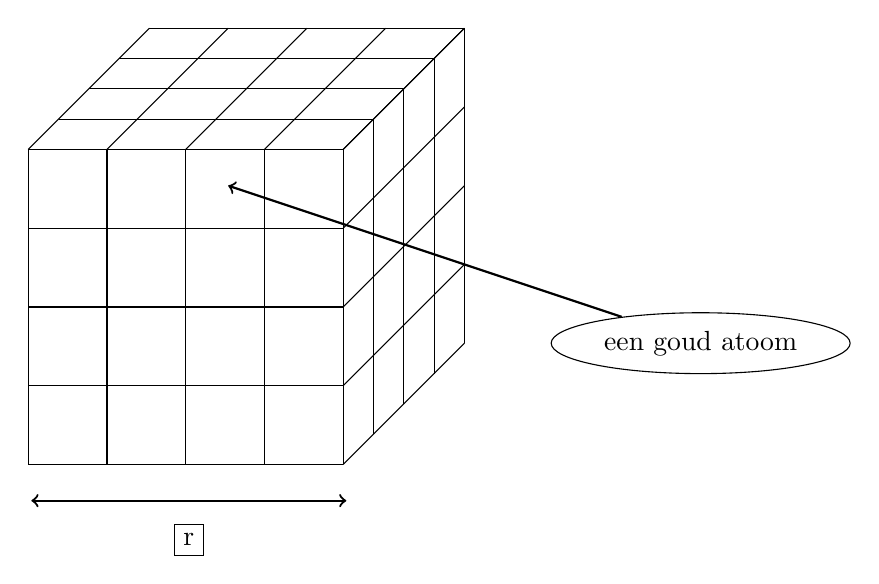
\begin{tikzpicture}
\foreach \x in{0,...,4}
{   \draw (0,\x ,4) -- (4,\x ,4);
    \draw (\x ,0,4) -- (\x ,4,4);
    \draw (4,\x ,4) -- (4,\x ,0);
    \draw (\x ,4,4) -- (\x ,4,0);
    \draw (4,0,\x ) -- (4,4,\x );
    \draw (0,4,\x ) -- (4,4,\x );
}
\coordinate (eindpijl) at (1,2);
\node [draw,ellipse] (start) at (7,0) {een goud atoom};
\draw [->, thick] (start) -- (eindpijl);
\draw [<->, thick] (-1.5,-2) -- (2.5,-2);
\node [draw] (begin) at (0.5,-2.5) {r};
\end{tikzpicture}
\end{figure}

De molaire massa van goud is \SI{197}{\gram\per\mol} en de dichtheid is 
\SI{19.3}{\gram\per\cubic\centi\meter}


$n = \frac{m}{M} = \frac{\rho \cdot V}{M} = 0,098 [mol]\\
N = n \cdot N_{A} = 5.9\cdot10^{22}$ \\
Er zijn $5,9\cdot 10^{22}$ atomen in de kubus van \SI{1.0}{\cubic\centi\meter} aanwezig.
$V = r^3 $ en $V^{'} = a^{3}$ \\Waar $V^{'} = \frac{V}{N}$ het volume wat een goudatoom in het rooster inneemt.\\
$a = \sqrt[3]{\frac{V}{N}} = 2,56\cdot 10^{-8} cm \approx 2,6 \cdot 10^{-10} m$
De straal van het atoom is dus $\approx$ \SI{1e-10}{\meter}.

\question
Welke energie is nodig om met elektronen de innerlijke structuur van \\
I. atomen te onderzoeken?\\

II. protonen en neutronen te onderzoeken?\\
Bedenk dat de alle materie een golflengte heeft (de Broglie \footnote{zie routenet: \url{http://www.hisparc.nl/docent-student/lesmateriaal/routenet}}
) en dat de resolutie voor waarneming afhangt van de golflengte van het deeltje wat voor detectie moet zorgen.

I. Om de structuur van atomen te onderzoeken heb je een resolutie nodig van \SI{e-10}{\meter}
Er geldt (voor atomen):\\
$p = \frac{h}{\lambda} = \frac{6,626\cdot 10^{-34}}{10^{-10}} = 6,626 \cdot 10^{-24} kgm/s$\\
$E_{kin} = \frac{p^2}{2m} = 150 eV$
Het gaat hier om niet relativistische elektronen omdat ze energie minder is dan de rustenergie van elektronen.

II. Kerndeeltjes hebben afmetingen kleiner dan \SI{1e-15}{\meter}. 
Er geldt (voor kerndeeltjes):\\
$p = \frac{h}{\lambda} = \frac{6,626\cdot 10^{-34}}{10^{-15}} = 6,626 \cdot 10^{-29} kgm/s$\\
$E= \sqrt{p^{2}c^{2}+m_0^{2}c^{4}} \approx pc = 1,24 GeV$
Elektronen zijn met deze energie relativistisch. 


\question
Doordat we de afmetingen van neutronen en protonen weten, kunnen we schatten wat 
de massa is van het deeltje wat voor de interactie tussen die twee zorgt.
Gebruik hierbij de onzekerheidsrelatie van Heisenberg en de tijd die een deeltje
nodig heeft om een afstand in de orde van grootte van een kerndeeltje af te leggen.
De afstand tussen twee nucleonen is in de orde van \SI{e-15}{m}.

\makelines{4} 
 
$r = c \cdot \Delta t \rightarrow \Delta t = \frac{r}{c} = \frac{10^{-15}}{3,0\cdot 10^{8}}= 3,34\cdot 10^{-24} s$

$\Delta E \cdot \Delta t \geq \hbar \rightarrow \Delta E = \frac {\hbar}{\Delta t} = 197 MeV$

Waarin: $\hbar$ is $ \frac{h}{2\pi}$
 

De onzekerheidsrelatie voor een afstand van \SI{e-15}{m} geeft een afwijking in de energie van 
ongeveer \SI{200}{\mega\electronvolt}. Een deeltje wat zorgt voor een interactie tussen 
twee nucleonen zou dus een massa moeten hebben in de orde grootte van \SI{200}{\mega\electronvolt},
maar kan slechts \SI{e-24}{\second} bestaan. Yukawa voorspelde het $\pi$ -meson en Powell ontdekte het deeltje 
met een massa van \SI{140}{\mega\electronvolt}. Yukawa kreeg in 1949 de Nobelprijs.

\begin{figure}
\caption{ Feynman voorstelling van sterke kernkracht door pionen.}
\tikzset{
particle/.style={thick,draw=blue, postaction={decorate},
    decoration={markings,mark=at position .5 with {\arrow[blue]{triangle 45}}}}
    }
\subfloat[proton, neutron interactie met uitwisseling van $\pi^0$.]
{

\begin{tikzpicture}

\coordinate(p1) at (2,2);
\coordinate(aux1) at (2,2);
\coordinate(p2) at (0,4);

\coordinate(n1) at (6,0);
\coordinate(n2) at (6,4);
\coordinate(aux2) at (4,2);

\draw[particle] (0, 0) node [left] {p} -- (p1) ;
\draw[particle] (p1) -- (p2) node [left] {p};
\draw[particle] (n1) node [right] {n} -- (aux2) ;
\draw[particle] (aux2) -- (n2) node [right] {n};
\draw[dotted, thick] (aux1) -- (aux2) node [midway, above] {$\pi^0$};
%\draw[gluon] (aux1) -- node[label=right:$\gamma$] {} (aux2);

\end{tikzpicture}
}
\subfloat[Interactie tussen p en n onder uitwisseling van een $pi^{+}$]
{
\tikzset{
particle/.style={thick,draw=blue, postaction={decorate},
    decoration={markings,mark=at position .5 with {\arrow[blue]{triangle 45}}}}
    }
\begin{tikzpicture}

\coordinate(p1) at (2,2);
\coordinate(aux1) at (2,2);
\coordinate(p2) at (0,4);

\coordinate(n1) at (6,0);
\coordinate(n2) at (6,4);
\coordinate(aux2) at (4,2);

\draw[particle] (0,0) node [left] {p}  -- (p1) ;
\draw[particle] (p1) -- (p2) node [left] {n};
\draw[particle] (n1) node [right] {n} -- (aux2) ;
\draw[particle] (aux2) -- (n2) node [right] {p};
\draw[dotted, thick] (aux1) -- (aux2) node [midway, above] {$\pi^+$};
%\draw 
%\draw[gluon] (aux1) -- node[label=right:$\gamma$] {} (aux2);
\end{tikzpicture}
}

\label{fig:Pion_feynman}
\end{figure}

\section{ Versnellers}

In de LHC guide die je kunt downloaden van de Cern site vind je
informatie over de LHC en over de bundels protonen die deze versneller
tot dichtbij de lichtsnelheid en vervolgens laat botsen in detectoren
zoals CMS en ATLAS. Om ons een betere voorstelling te kunnen maken gaan
we even rekenen aan de eigenschappen van de protonen bundels in de LHC.

\question
Vergelijk de dichtheid in een protonenbundel in de LHC met de dichtheid van zuurstof en goud 
(beide bij kamertemperatuur). Een bundel protonen is een cilinder met een lengte 
van \SI{15}{\centi\meter} en een straal van \SI{17e-6}{m}, met zo'n \SI{e11}{} protonen.
(We rekenen niet met de relativistische effecten doordat de protonen zwaarder worden.)
 
\makelines{4} 

De dichtheid van goud kun je opzoeken in Binas, deze geeft een waarde van 
$\rho$ is \SI{19.3}{\kilogram\per\cubic\meter}, wat je kunt omrekenen naar
een $\rho$ van \SI{19.3}{\gram\per\cubic\centi\meter}. 
Bij zuurstof gebruiken we dat er een mol zuurstof in \SI{22.4}{\liter} gaat.

$\rho_0 = \frac{n \cdot M}{V} = \frac {1 mol \cdot 16 g/mol}{22,4 L} = 7,14 \cdot 10^{-4} g/cm^{3} $

Voor de dichtheid in de bundel geldt:\\

$\rho_{bundel} = \frac{m}{V} = \frac{n_{p} \cdot m_{p}}{\pi \cdot r^2 \cdot l} \approx 1,23 \cdot 10^{-3} g/cm^{3}$


De dichtheid van de bundel zit tussen een gas en vaste stof in.






\begin{figure}[h]
\centering
\begin{tikzpicture}
\draw [thick] (0, 0) circle (0.6 cm) node {\huge+};
%\draw [dashed] (0,0) circle (4 cm);
\draw [thick] (85:4cm) circle (.4 cm) node {$\mu^-$};
\draw [dashed,thick] (95:4cm) arc (95:435:4cm); 
\draw[thick,->] (0,0) -- (85:1.6cm) node [right] {$\vec{F}_{\mu,p}$};
\draw[thick,->] (85:4 cm) -- (85:2.4cm) node [left]{$\vec{F}_{p,\mu}$};
\end{tikzpicture}
\caption{Muon waterstofatoom}
\label{fig:Muon_waterstofatoom}
\end{figure}

\begin{figure}
\centering
\foreach \n in{6}{%
\begin{tikzpicture}
 \begin{axis}[axis equal,
    xmin=-3,xmax=3,
    ymin=-3,ymax=3,
    axis lines=none]
 \addplot[samples=400,domain=0:2*pi,thick] ({(2+.3*cos(deg(\n*x)))*cos(deg(x))},{(2+.3*cos(deg(\n*x)))*sin(deg(x))});
 \addplot[samples=40,domain=0:2*pi,dashed] ({2*cos(deg(x))},{2*sin(deg(x))});
 \node at (axis cs:0,0){$n=\n$};
\end{axis}
\end{tikzpicture}
}
\end{figure}


\end{questions} 
\end{document}
